% figures-es/ai-build-buy.tex
% Standalone TikZ: matriz 2x2 Construir vs Comprar vs API para IA (ch.17 estrategia de datos e IA).
% Ejes: horizontal = especificidad de tarea (genérica -> propietaria);
%        vertical   = ventaja de datos propios (baja -> alta).
% Compilado a figures-es/ai-build-buy.pdf via tools/build-figures-es.sh.
\documentclass[tikz,border=4pt]{standalone}
\usepackage{tikz}
\usetikzlibrary{arrows.meta,positioning}

\definecolor{vcblue}{HTML}{1A5276}
\definecolor{vcteal}{HTML}{0E6655}
\definecolor{vcgray}{HTML}{4D4D4D}

\begin{document}
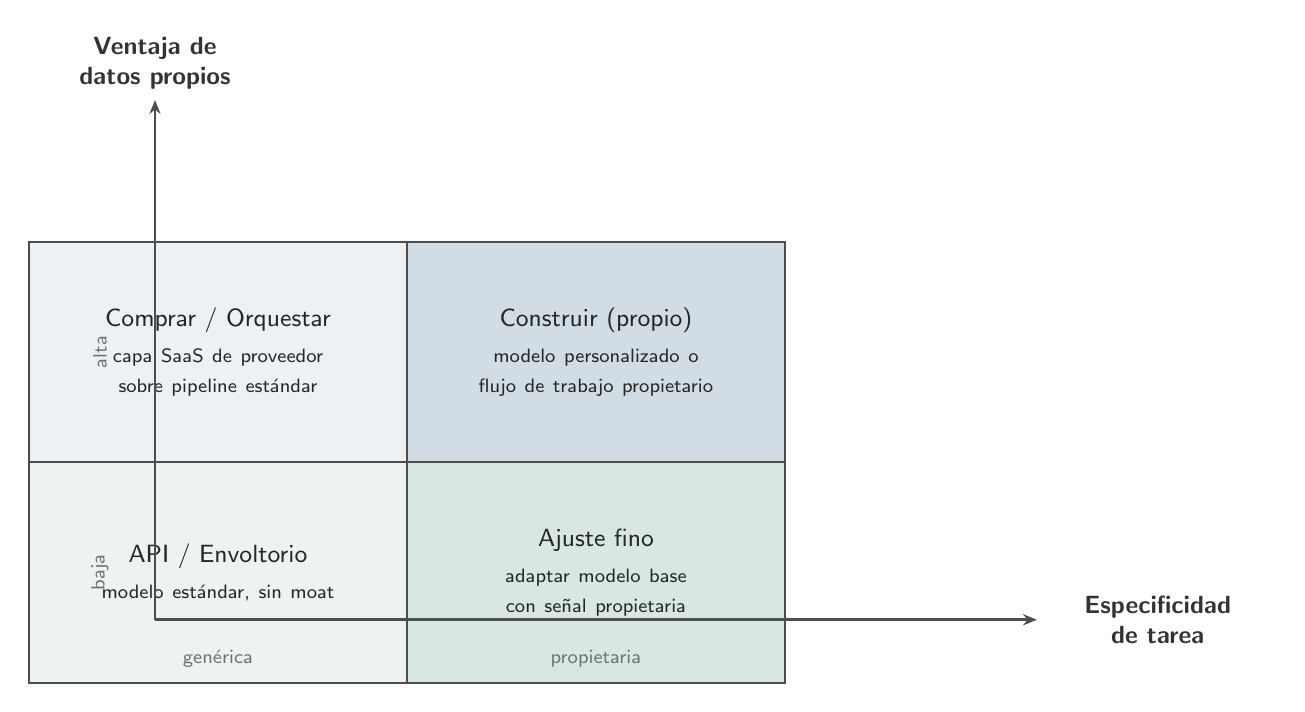
\begin{tikzpicture}[
  cell/.style={draw=vcgray, line width=0.7pt, align=center, text width=40mm,
               minimum width=48mm, minimum height=28mm, font=\sffamily\small, text=black!85},
  axislbl/.style={font=\sffamily\small\bfseries, text=black!80, align=center},
  sublbl/.style={font=\sffamily\scriptsize, text=black!55, align=center},
  arr/.style={-{Stealth[length=5pt,width=4pt]}, vcgray, line width=1pt},
]

% Celdas de cuadrante (SO, SE, NO, NE). El subtexto se ajusta mediante text width (sin saltos de línea anidados).
\node[cell, fill=vcteal!8]  (sw) at (0,0)      {API / Envoltorio\\[2pt]{\scriptsize modelo estándar, sin moat}};
\node[cell, fill=vcteal!16] (se) at (48mm,0)   {Ajuste fino\\[2pt]{\scriptsize adaptar modelo base con señal propietaria}};
\node[cell, fill=vcblue!8]  (nw) at (0,28mm)   {Comprar / Orquestar\\[2pt]{\scriptsize capa SaaS de proveedor sobre pipeline estándar}};
\node[cell, fill=vcblue!20] (ne) at (48mm,28mm){Construir (propio)\\[2pt]{\scriptsize modelo personalizado o flujo de trabajo propietario}};

% Flechas de ejes
\draw[arr] (-8mm,-6mm) -- (-8mm,60mm)
  node[axislbl, above, text width=30mm] {Ventaja de\\datos propios};
\draw[arr] (-8mm,-6mm) -- (104mm,-6mm)
  node[axislbl, right, text width=28mm] {Especificidad\\de tarea};

% Etiquetas de marcas del eje
\node[sublbl] at (0,-11mm)   {genérica};
\node[sublbl] at (48mm,-11mm){propietaria};
\node[sublbl, rotate=90] at (-15mm,0)    {baja};
\node[sublbl, rotate=90] at (-15mm,28mm) {alta};

\end{tikzpicture}
\end{document}
